\newSection{Experiments}

\begin{frame}[t]{Datasets}
    \textbf{Real:} \emph{HiSa} \& \emph{HiDa}
    \vspace{5pt}
    \textbf{Synthetic:} \emph{USC-HairSalon}\cite{Hu2015SingleviewHM}
    \begin{itemize}
        \item \textbf{343} 3D hair models, multiple views.
        \item \emph{HairStep} (strand + depth maps), ground-truth fields.
    \end{itemize}
\end{frame}


\begin{frame}[t]{Evaluation Metrics}
    \textbf{Quantitative Evaluation:}
    \begin{itemize}
        \item \textbf{Real Data:}
        \begin{itemize}
            \item \emph{HairSale:} Mean angle error of strand growth directions.
            \item \emph{HairRida:} Accuracy of predicted depth ordering relative to ground truth.
        \end{itemize}
        \item \textbf{Synthetic Data:}
        \begin{itemize}
            \item \emph{Orientation Error:} $L2$ error between predicted and ground-truth orientation fields.
            \item \emph{Occupancy Precision:} Precision of predicted occupancy field compared to ground truth.
        \end{itemize}
    \end{itemize}
    \vspace{4pt}
    \textbf{Qualitative Evaluation:}
    \begin{itemize}
        \item \emph{Visual Quality:} Visual assessment of reconstruction results.
        \item \emph{User Study} Limited user evaluations of result quality.
    \end{itemize}
\end{frame}



\begin{frame}[t]{Evaluation Metrics -- HairSale}
    \textbf{HairSale: Mean Angle Error of Growing Direction}
    \begin{equation*}
        \text{HairSale} = \frac{1}{K} \sum_{i} \arccos\left( V(O_r(x_i)) \cdot V(O_{gt}(x_i)) \right)
    \end{equation*}
    \begin{itemize}
        \item \textbf{Components:}
        \begin{itemize}
            \item \(U\): Intersected region of rendered mask and ground-truth.
            \item \(K\): Total pixels in \(U\).
            \item \(V(O_r(x_i))\): Unit vector at pixel \(x_i\) in rendered strand map.
            \item \(V(O_{gt}(x_i))\): Unit vector at pixel \(x_i\) in ground-truth strand map.
        \end{itemize}
        \item \textbf{Range:} 0 to 180 degrees.
    \end{itemize}
\end{frame}


\begin{frame}[t]{Evaluation Metrics -- HairRida}
    \textbf{HairRida: Relative Depth Accuracy}
    \begin{equation*}
        \text{HairRida} = \frac{1}{Q} \sum_{i} \max(0, r_i \cdot \text{sign}(D_r(p_{i1}) - D_r(p_{i2})))
    \end{equation*}
    \begin{itemize}
        \item \textbf{Components:}
        \begin{itemize}
            \item \(U\): Intersected region of rendered mask and ground-truth.
            \item \(Q\): Total number of pixel pairs in \(U\).
            \item \(r_i\): Ground-truth relative depth order.
            \item \(D_r(p_{i1})\), \(D_r(p_{i2})\): Depth values at pixel pair \(p_{i1}\) and \(p_{i2}\) in rendered depth map.
        \end{itemize}
    \end{itemize}
\end{frame}


\begin{frame}[t]{Evaluation Metrics -- HairSale \& HairRida}
    \begin{figure}
        \centering
        \includegraphics[width=0.95\textwidth]{assets/figures/eval/metrics/metrics.png}
        \caption{\textit{HairSale} and \textit{HairRida}.}
    \end{figure}
\end{frame}

\begin{frame}{Evaluation Metrics -- Qualitative}
    \begin{figure}
        \centering
        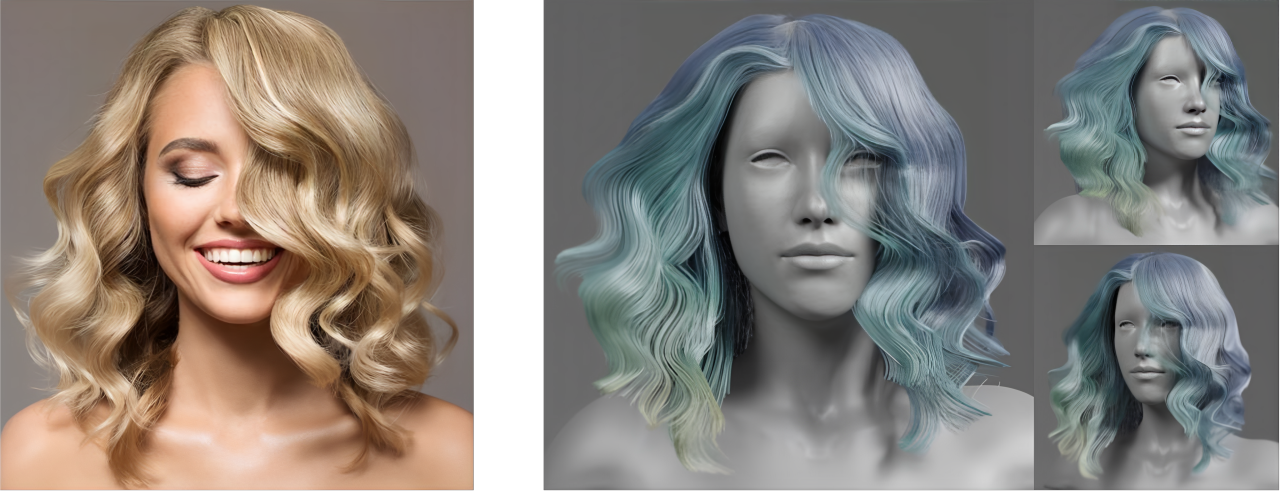
\includegraphics[width=0.9\textwidth]{assets/figures/eval/metrics/input-output.png}
    \end{figure}
\end{frame}


\begin{frame}[t]{Experimets}
    \emph{HairStep Extraction:}
    \begin{itemize}
        \item Extraction of strand maps.
        \item Extraction of depth maps.
    \end{itemize}
    \emph{Baseline Comparisons:}
    \begin{itemize}
        \item Single-view 3D hair modeling.
        \item Intermediate representation effectiveness.
    \end{itemize}
\end{frame}


\begin{frame}{HairStep Extraction -- Strand Maps}
    \begin{figure}
        \centering
        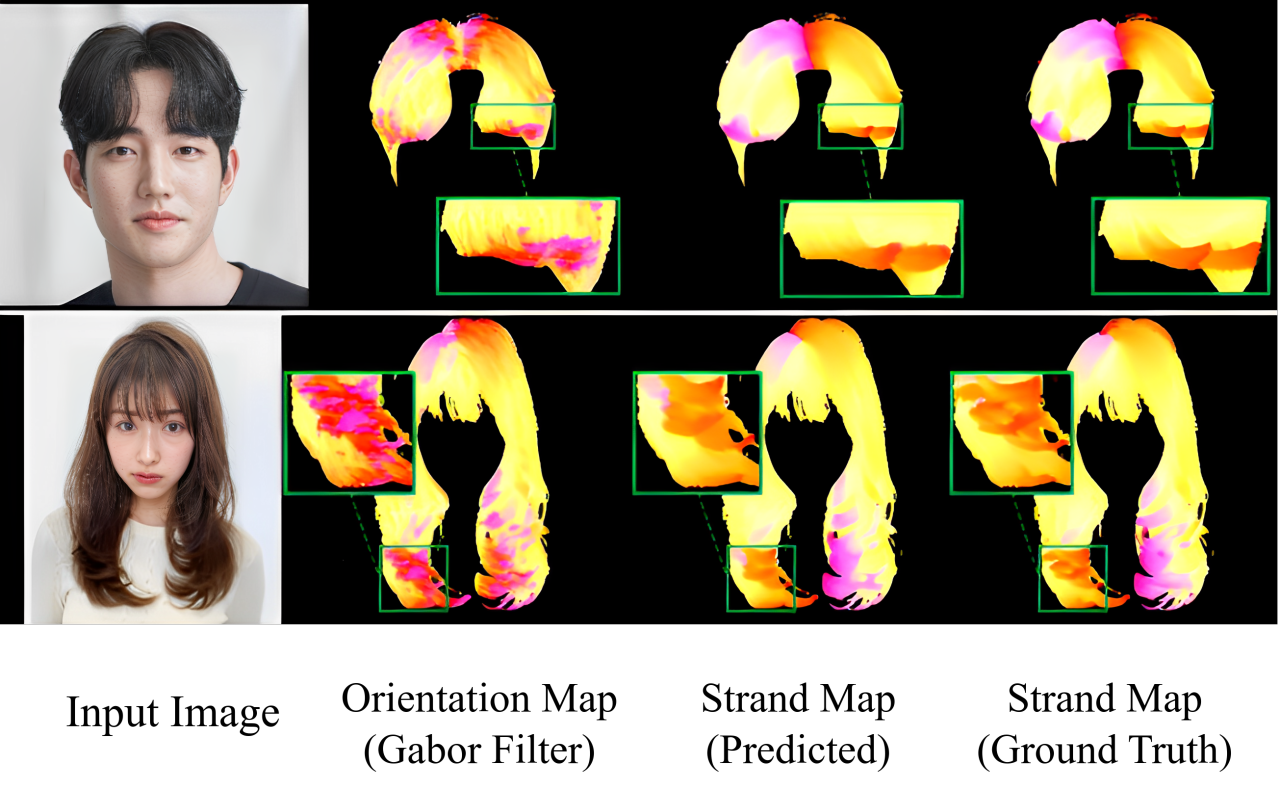
\includegraphics[width=0.65\textwidth]{assets/figures/eval/hairsale/strand-prediction-comparison.png}
        \caption{Qualitative comparisons on orientation/strand maps.}
    \end{figure}
\end{frame}


\begin{frame}{HairStep Extraction -- Strand Maps}

    \begin{table}[]
        \renewcommand{\arraystretch}{1.5}
        \centering
        \small
        \begin{tabularx}{0.55\textwidth}{
            >{\raggedright\arraybackslash}X
            >{\raggedright\arraybackslash}p{3.5cm}
        }
            \hline
            \rowcolor{myLightBlue}
            \textbf{Method} & \textbf{HairSale $\downarrow$ (Undirected)} \\ \hline
            Gabor Filters & 18.4 \\ \hline
            HairStep & \textbf{14.2} \\ \hline
        \end{tabularx}
        \caption{Undirected \textit{HairSale} comparison: \textit{HairStep} performs 22.8\% better than Gabor filters.}
    \end{table}
\end{frame}


\begin{frame}[t]{HairStep Extraction -- Depth Maps}
    \begin{figure}
        \centering
        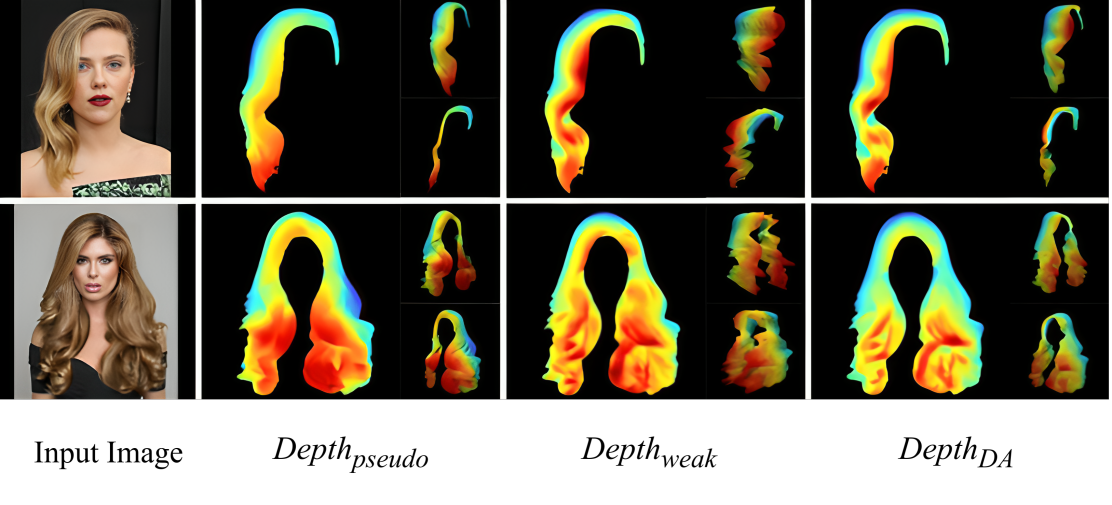
\includegraphics[width=0.9\textwidth]{assets/figures/eval/hairrida/depth-comparison.png}
        \caption{Qualitative comparisons on depth maps.}
    \end{figure}
\end{frame}


\begin{frame}[t]{HairStep Extraction -- Depth Maps}
    \begin{itemize}
        \item \textbf{Depth$_{pseudo}$:} Depth estimation using pseudo labels from the synthetic domain.
        \item \textbf{Depth$_{weak}$:} Weakly supervised depth estimation using ordinal labels.
        \item \textbf{Depth$_{DA}$:} Domain-adaptive depth estimation method.
    \end{itemize}  \begin{table}[]
        \renewcommand{\arraystretch}{1.5}
        \centering
        \small
        \begin{tabularx}{0.75\textwidth}{
            >{\raggedright\arraybackslash}X
            >{\raggedright\arraybackslash}p{3.5cm}
            >{\raggedright\arraybackslash}p{3.5cm}
        }
            \hline
            \rowcolor{myLightBlue}
            \textbf{Method} & \textbf{HairRida $\uparrow$} & \textbf{L1 Loss $\downarrow$} \\ \hline
            $Depth_{pseudo}$ & 80.47\% & - \\ \hline
            $Depth_{weak}$ & 85.17\% & 0.2470/3.125 \\ \hline
            $Depth_{DA}$ & \textbf{85.20\%} & \textbf{0.1768/0.1188} \\ \hline
        \end{tabularx}
        \caption{Relative depth accuracy and L1 loss comparison:}
    \end{table}
\end{frame}

\begin{frame}[t]{Baseline Comparisons -- Single-View 3D Hair Modeling}
    \textbf{Methods Compared:}
    \begin{itemize}
        \item HairNet~\cite{Zhou2018SingleViewHR}
        \item DynamicHair~\cite{Yang2019DynamicHM}
        \item NeuralHDHair~\cite{wu2022neuralhdhair}
        \item NeuralHDHair* + HairStep (Authors' implementation of NeuralHDHair)
    \end{itemize}
\end{frame}

\begin{frame}{Single-View 3D Hair Modeling -- Qualitative Comparisons (1/2)}
    \begin{figure}
        \centering
        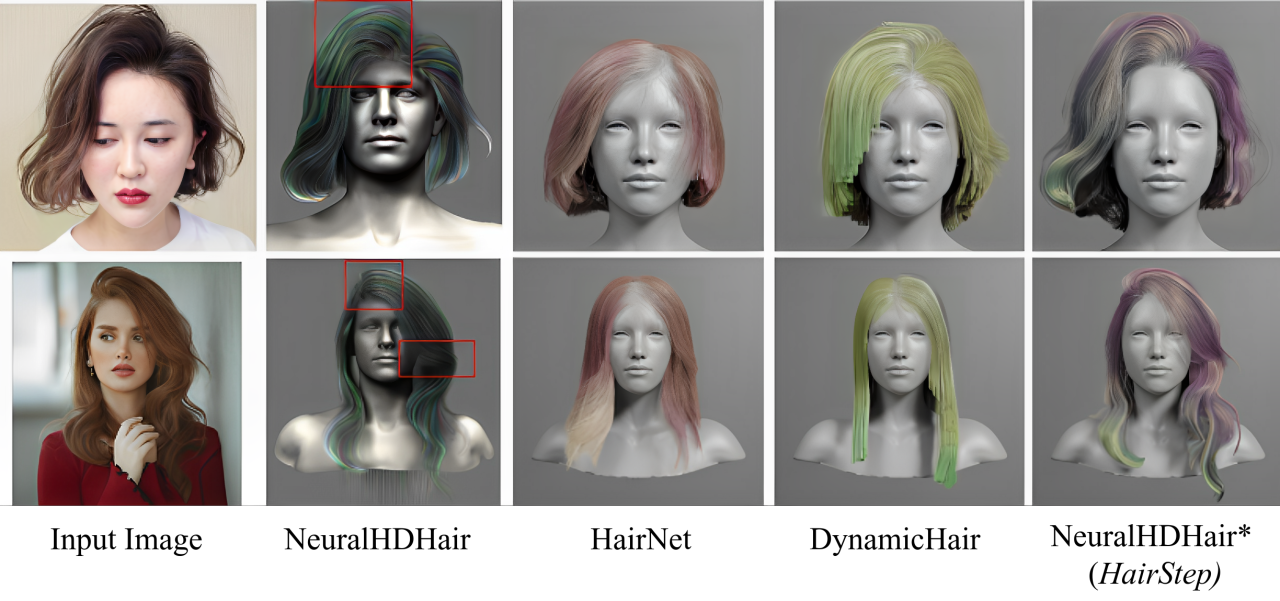
\includegraphics[width=0.7\textwidth]{assets/figures/eval/existing-methods-vis-comparison-1.png}
        \caption{Qualitative comparisons with baselines.}
    \end{figure}
\end{frame}

\begin{frame}{Single-View 3D Hair Modeling -- Qualitative Comparisons (2/2)}
    \begin{figure}
        \centering
        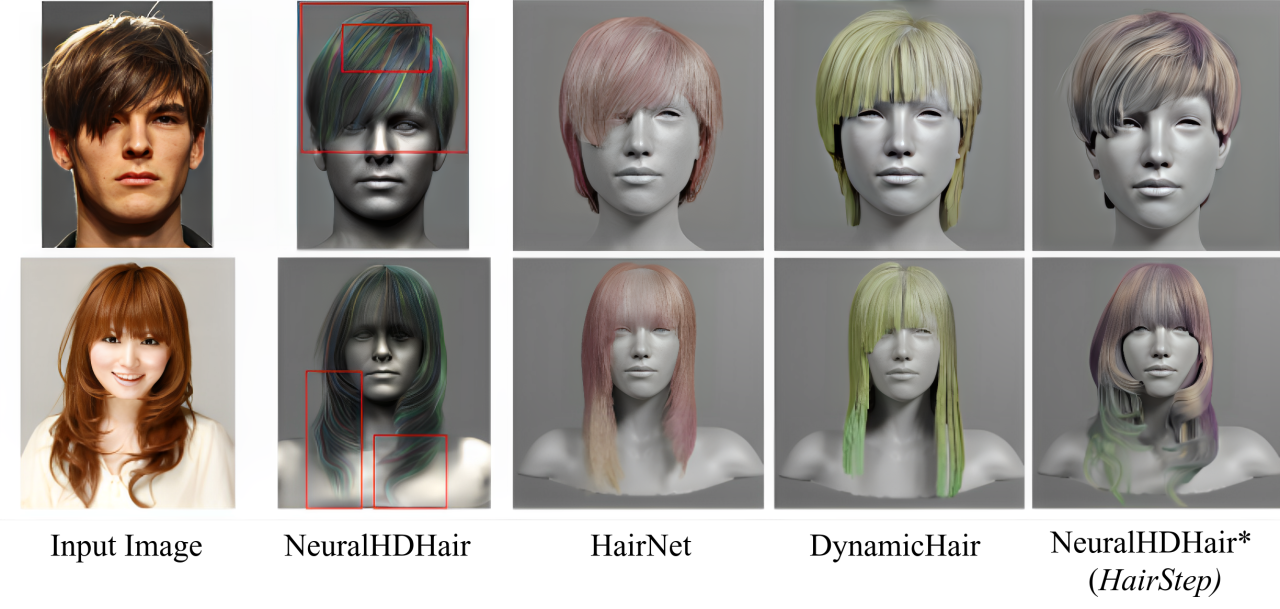
\includegraphics[width=0.7\textwidth]{assets/figures/eval/existing-methods-vis-comparison-2.png}
        \caption{Qualitative comparisons with baselines.}
    \end{figure}
\end{frame}

\begin{frame}[t]{Single-View 3D Hair Modeling -- Observations}
    \begin{itemize}
        \item HairNet and DynamicHair produce coarse shapes, struggle with complex styles.
        \item NeuralHDHair fails with sharp depth variations and complex growth patterns.
        \item Gabor filter orientation maps lack detail for accurate 3D modeling.
    \end{itemize}
\end{frame}

\begin{frame}[t]{Baseline Comparisons -- Representation Effectiveness}
    \begin{itemize}
        \item \textbf{Objective:} Assess how different representations impact 3D hair reconstruction.
        \item \textbf{Representations Compared:}
        \begin{itemize}
            \item Orientation Map
            \item Strand Map
            \item \textit{HairStep} (Strand Map + Depth Map)
        \end{itemize}
        \item \textbf{Methods Compared:}
        \begin{itemize}
            \item HairNet~\cite{Zhou2018SingleViewHR}
            \item DynamicHair~\cite{Yang2019DynamicHM}
            \item NeuralHDHair* (Authors' implementation of NeuralHDHair~\cite{wu2022neuralhdhair})
        \end{itemize}
    \end{itemize}
\end{frame}

% Second frame: Quantitative Results and Observations
\begin{frame}[t]{Representation Effectiveness -- Synthetic Data}
    \begin{table}[h]
        \centering
        \small
        \renewcommand{\arraystretch}{1.2}
        \begin{tabular}{l|c|c}
            \hline
            \rowcolor{myLightBlue}
            Method & Orientation Error $\downarrow$ & Occupancy Accuracy $\uparrow$ \\
            \hline
            HairNet (Orientation Map) & 0.02349 & -- \\
            HairNet (Strand Map) & 0.02206 \textcolor{blue}{(-6.1\%)} & -- \\
            HairNet (\textbf{HairStep}) & \textbf{0.02184} \textcolor{blue}{(-7.0\%)} & -- \\
            \midrule
            DynamicHair (Orientation Map) & 0.1352 & 78.19$\%$ \\
            DynamicHair (Strand Map) & 0.1185 \textcolor{blue}{(-12.4\%)} & 79.62$\%$ \\
            DynamicHair (\textbf{HairStep}) & \textbf{0.1174} \textcolor{blue}{(-13.2\%)} & \textbf{79.78$\%$} \\
            \midrule
            NeuralHDHair* (Orientation Map) & 0.1324 & 82.59$\%$ \\
            NeuralHDHair* (Strand Map) & 0.0722 \textcolor{blue}{(-41.7\%)} & 84.18$\%$ \\
            NeuralHDHair* (\textbf{HairStep}) & \textbf{0.0658} \textcolor{blue}{(-50.3\%)} & \textbf{86.77$\%$} \\
            \bottomrule
        \end{tabular}
        \caption{Quantitative comparisons on the USC-HairSalon dataset using different representations.}
        \label{tab:representation_effectiveness_synthetic}
    \end{table}
\end{frame}

% Third frame: Quantitative Results on Real Data
\begin{frame}[t]{Representation Effectiveness -- Real Data}
    \begin{table}[h]
        \centering
        \small
        \renewcommand{\arraystretch}{1.1}
        \begin{tabular}{l|c|c|c}
            \hline
            \rowcolor{myLightBlue}
            Method & IoU $\uparrow$ & \textit{HairSale} $\downarrow$ & \textit{HairRida} $\uparrow$ \\
            \hline
            HairNet (Orientation Map) & 57.15$\%$ & 31.97 & 75.65$\%$ \\
            HairNet (Strand Map) & 57.48$\%$ & 28.60 \textcolor{blue}{(-10.5\%)} & 74.81$\%$ \\
            HairNet (HairStep) & 57.01$\%$ & \textbf{27.68} \textcolor{blue}{(-13.4\%)} & \textbf{74.97$\%$} \\
            \midrule
            DynamicHair (Orientation Map) & 56.39$\%$ & 32.66 & 74.08$\%$ \\
            DynamicHair (Strand Map) & 59.51$\%$ & \textbf{26.53} \textcolor{blue}{(-18.8\%)} & 73.42$\%$ \\
            DynamicHair (HairStep) & 59.14$\%$ & 27.51 \textcolor{blue}{(-15.8\%)} & \textbf{73.58$\%$} \\
            \midrule
            NeuralHDHair* (Orientation Map) & 77.56$\%$ & 19.60 & 70.67$\%$ \\
            NeuralHDHair* (Strand Map) & 77.60$\%$ & \textbf{16.00} \textcolor{blue}{(-18.4\%)} & 72.37$\%$ \\
            NeuralHDHair* (HairStep) & 77.22$\%$ & 16.36 \textcolor{blue}{(-16.5\%)} & \textbf{76.79$\%$} \\
            \bottomrule
        \end{tabular}
        \caption{Quantitative comparisons on real data using different representations.}
        \label{tab:representation_effectiveness_real}
    \end{table}
\end{frame}

\begin{frame}[t]{Representation Effectiveness -- Real Data (Qualitative)}
    \begin{figure}
        \centering
        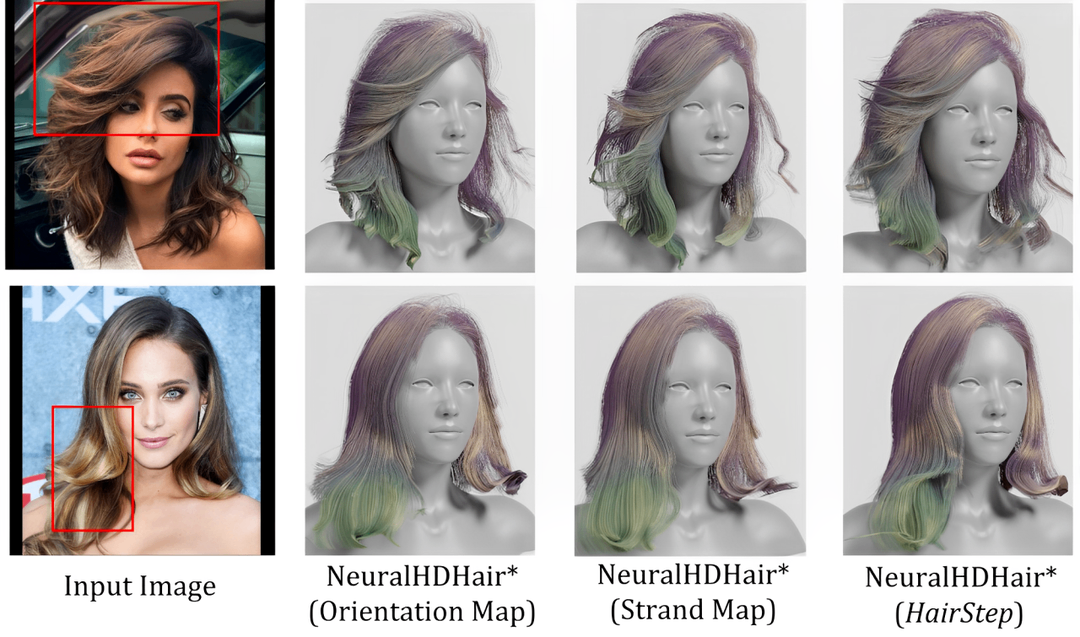
\includegraphics[width=0.6\textwidth]{assets/figures/eval/neuralhdhair.png}
        \caption{Qualitative results of NeuralHDHair* using orientation map, strand map, and HairStep, from left to right, respectively.}
    \end{figure}
\end{frame}

\begin{frame}[t]{Representation Effectiveness -- Observations}
    \textit{HairStep} benefits all methods on noth synthetic and real data.

    \vspace{5pt}

    \textbf{User Study:} Conducted on 10 randomly selected examples with 39 users.
    \begin{itemize}
        \item 64.87\% preferred HairStep.
        \item 21.28\% preferred strand map.
        \item 13.85\% preferred undirected orientation map.
    \end{itemize}
\end{frame}

% Slide 9: Ablation Studies
% Slide: Ablation Studies
\begin{frame}[t]{Ablation Studies}
    \textbf{Objective:} Evaluate the effect of different depth estimation methods on the final results.

    \vspace{5pt}
    \textbf{Methods:}
    \begin{itemize}
        \item \textbf{$C_0$}: Strand map + $Depth_{pseudo}$
        \item \textbf{$C_1$}: Strand map + $Depth_{weak}$
        \item \textbf{Full}: Strand map + $Depth_{DA}$
    \end{itemize}

    \begin{table}[h]
        \centering
        \small
        \renewcommand{\arraystretch}{1.2}
        \begin{tabularx}{0.75\textwidth}{
            >{\raggedright\arraybackslash}X
            >{\raggedright\arraybackslash}X
            >{\raggedright\arraybackslash}p{2.5cm}
            >{\raggedright\arraybackslash}p{2.5cm}
        }
            \hline
            \rowcolor{myLightBlue}
            Method & IoU $\uparrow$ & \textit{HairSale} $\downarrow$ & \textit{HairRida} $\uparrow$ \\
            \hline
            \textbf{$C_0$} & 77.75\% & 16.03 \textcolor{blue}{(-18.2\%)} & 73.57\% \\
            \textbf{$C_1$} & 77.11\% & 16.54 \textcolor{blue}{(-15.6\%)} & 75.80\% \\
            \textbf{Full}  & \textbf{77.22\%} & \textbf{16.36 \textcolor{blue}{(-16.5\%)}} & \textbf{76.79\%} \\
            \hline
        \end{tabularx}
        \caption{Quantitative ablation study on depth estimation methods.}
    \end{table}
\end{frame}

\begin{frame}[t]{Ablation Studies}
    \begin{figure}
        \centering
        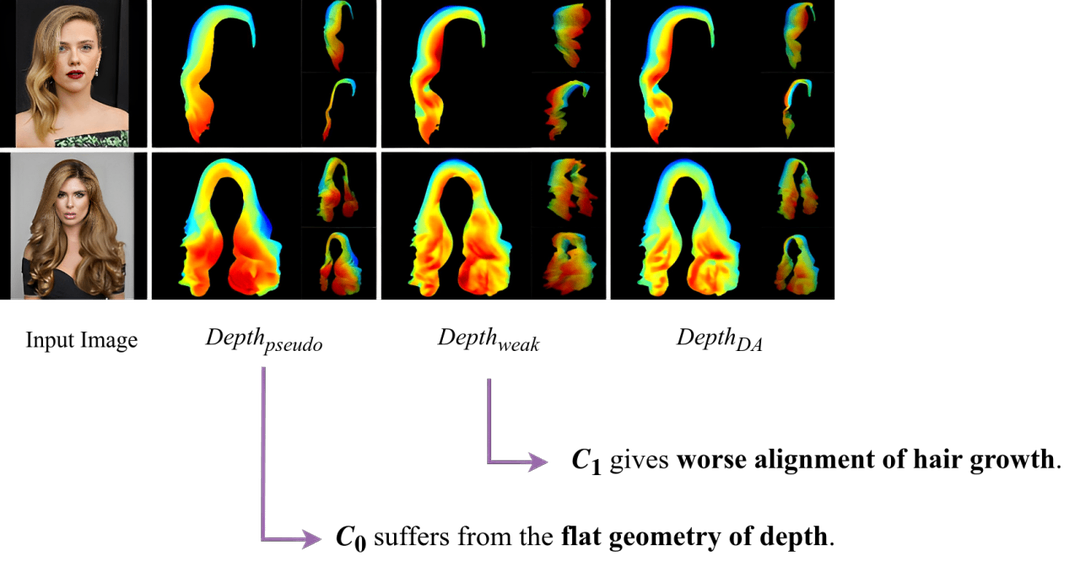
\includegraphics[width=0.8\textwidth]{assets/figures/eval/ablation/depth-comparison.png}
    \end{figure}
\end{frame}

\begin{frame}[t]{Ablation Studies -- Qualitative Comparison}
    \begin{figure}
        \centering
        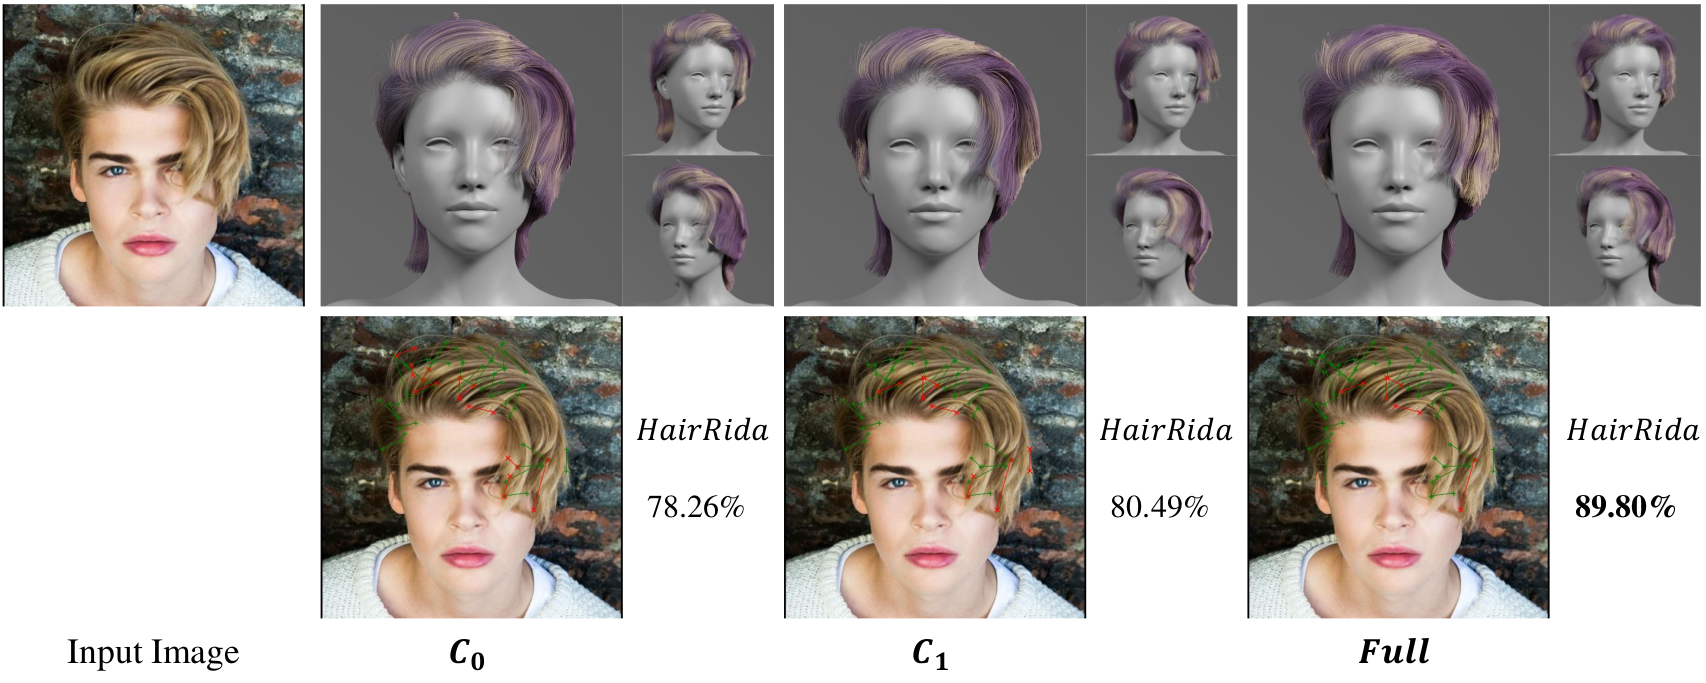
\includegraphics[width=0.8\textwidth]{assets/figures/eval/ablation/sample-1.png}
        \caption{From left to right: input images, results of $C_0$, $C_1$, and Full method. \textit{HairRida} visualized below each result with green/red lines for correct/incorrect predictions.}
    \end{figure}
\end{frame}
